% DA INCREMENTARE PER 
\paragraph{MD001 - Indice di Gulpease}\mbox{}\\[0,3cm]
\begin{table}[H]
	\centering
	\begin{tabular}{cccc}
	\rowcolor{greySWEight}
	\textcolor{white}{\textbf{Documento}} & 
	\textcolor{white}{\textbf{Abbreviazione}} &
	\textcolor{white}{\textbf{Valore Indice}}&
	\textcolor{white}{\textbf{Riscontro}}\\
	
	\textbf{Analisi dei Requisiti} & ADR & 60,3 & \textcolor{ForestGreen}{Ottimale} \\
	\textbf{Glossario} & GLO & 59,3 & \textcolor{ForestGreen}{Ottimale} \\
	\textbf{Piano di Qualifica} & PDQ & 55,9 & \textcolor{ForestGreen}{Ottimale} \\
	\textbf{Piano di Progetto} & PDP & 55,3 & \textcolor{ForestGreen}{Ottimale} \\
	\textbf{Norme di Progetto} & NDP & 56,6 & \textcolor{ForestGreen}{Ottimale} \\

	\end{tabular}
	\caption{Indice di Gulpease nel periodo di codifica}
\end{table}

\begin{figure}[H]
	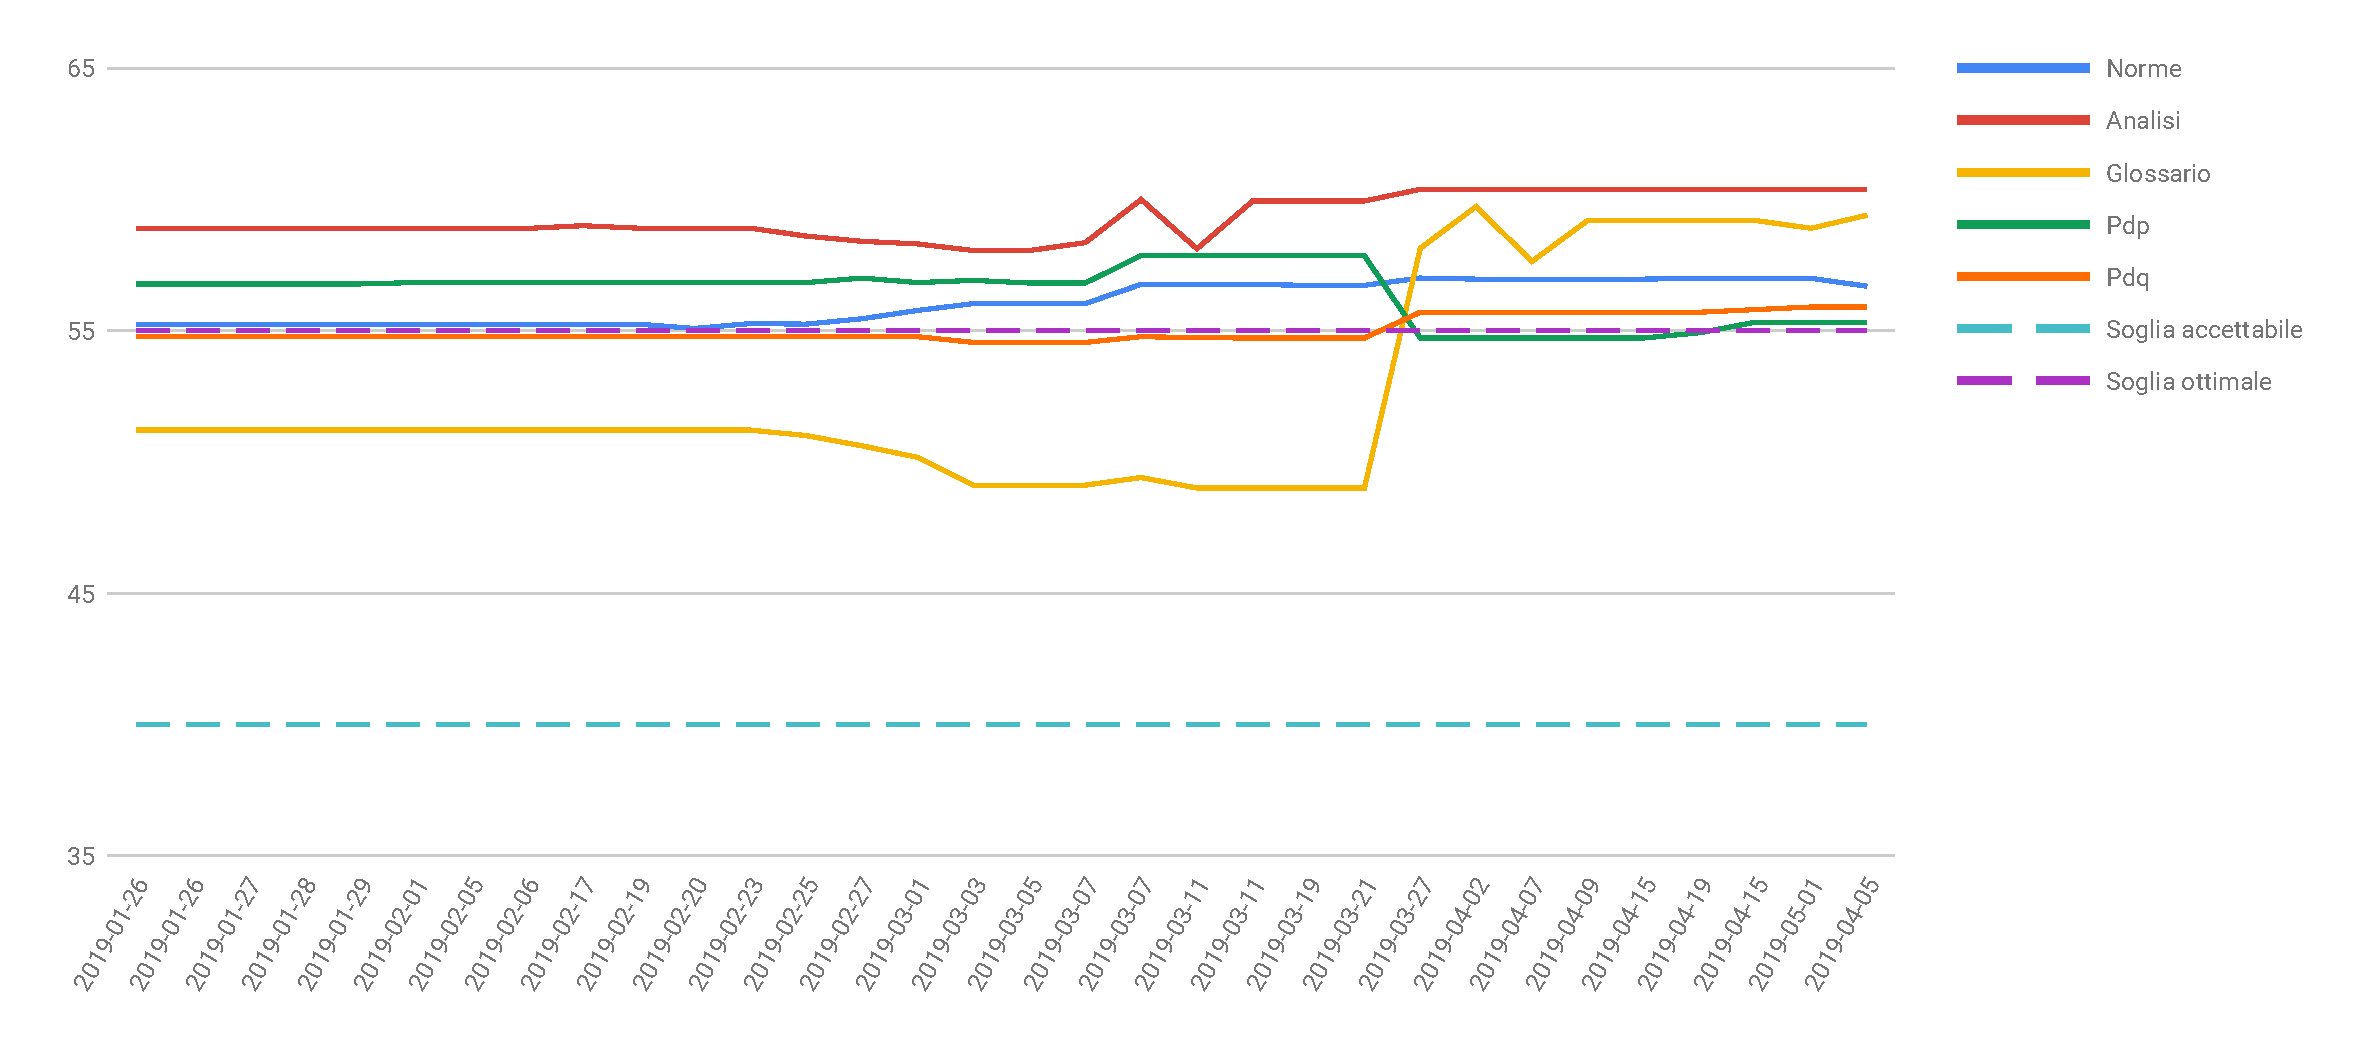
\includegraphics[width=1\linewidth]{sez/App_Esito/Approvazione/graph/indiceGulpeaseRA.pdf}
	\caption{Andamento dell'indice di Gulpease fino alla revisione di Approvazione}
\end{figure}
\newpage